\chapter{Capacity, Queues and Decisions under Uncertainty}

\begin{weekbox}
\textbf{Theme.} Variability costs capacity. Size staff against a service promise with queueing theory, check the
answer with simulation, and plan orders that are robust to forecast error instead of optimal for the average.\\
\textbf{Outcomes.} LO7.\quad \textbf{Tools.} SimPy, NumPy, PuLP.\\
\textbf{Data.} 6\,646 real orders (Online Retail II, Sept--Nov 2011): arrival times by hour and lines per order;
Mboa December order planning.\\
\textbf{Lab.} Erlang C staffing to an SLA; discrete-event simulation with time-varying arrivals and replications;
two-stage stochastic programming with VSS and EVPI.\\
\textbf{Deliverable.} Lab notebook. \textbf{CA3} (optimisation and simulation) follows this week.
\end{weekbox}

\begin{timetable}
0:00--0:20 & Briefing & ``Pickers are 70\% busy on average. Why do customers complain that orders leave late?''\\
0:20--1:10 & Concepts & Utilisation and waiting, M/M/1, M/M/$c$, Erlang C, SLAs, DES, flaw of averages, SAA\\
1:10--2:40 & Guided lab & Lab 6, Steps 1--3 (break at 1:55)\\
2:40--3:40 & Challenge & Exercises 6.3--6.8\\
3:40--4:00 & Debrief & What staffing plan would you sign off, and what service does it buy?\\
\end{timetable}

\section{Why queues form}
A queue forms whenever work arrives faster than it is served, \emph{even briefly}. Because arrivals and service times
vary, a resource that is busy 80\% of the time on average is overwhelmed some of the time and idle some of the time,
and the idle time cannot be stored for later.

\begin{definition}{Queueing notation}
Kendall's notation A/S/$c$ gives the arrival process, the service-time distribution and the number of servers
(M = Markovian, i.e.\ Poisson arrivals or exponential service; G = general). $\lambda$ is the arrival rate,
$\mu$ the service rate per server, $\rho=\lambda/(c\mu)$ the utilisation, and $a=\lambda/\mu$ the offered load in
\emph{Erlangs} (busy servers needed on average).
\end{definition}

\begin{keyformula}{Single and multiple servers}
M/M/1: $\quad L=\dfrac{\rho}{1-\rho},\quad W=\dfrac{1}{\mu-\lambda},\quad W_q=\dfrac{\rho}{\mu-\lambda}$.\\[4pt]
M/M/$c$, Erlang C (probability an arrival waits):
\[ C(c,a)=\frac{\dfrac{a^c}{c!}\dfrac{c}{c-a}}{\sum_{k=0}^{c-1}\dfrac{a^k}{k!}+\dfrac{a^c}{c!}\dfrac{c}{c-a}},\qquad
W_q=\frac{C(c,a)}{c\mu-\lambda},\qquad P(W_q\le t)=1-C(c,a)\,e^{-(c\mu-\lambda)t}. \]
Non-exponential service (Allen--Cunneen): $W_q^{G/G/c}\approx W_q^{M/M/c}\cdot\dfrac{c_a^2+c_s^2}{2}$, with $c^2$ the squared
coefficient of variation.
\end{keyformula}

\begin{figure}[H]
\centering
\begin{tikzpicture}
\begin{axis}[width=8.6cm,height=5.0cm,xmin=0,xmax=1,ymin=0,ymax=20,axis lines=left,
  xlabel={utilisation $\rho$},ylabel={mean wait $W_q$ (in service times)},
  tick label style={font=\scriptsize},label style={font=\scriptsize},legend style={font=\scriptsize,draw=none,at={(0.03,0.97)},anchor=north west}]
\addplot[navy,thick,domain=0:0.953,samples=120] {x/(1-x)};
\addplot[orange,thick,dashed,domain=0:0.976,samples=120] {0.5*x/(1-x)};
\legend{M/M/1 ($c_s^2=1$),M/D/1 ($c_s^2=0$)}
\draw[slate,dotted] (axis cs:0.8,0)--(axis cs:0.8,4)--(axis cs:0,4);
\draw[slate,dotted] (axis cs:0.9,0)--(axis cs:0.9,9)--(axis cs:0,9);
\end{axis}
\end{tikzpicture}
\caption{Waiting explodes as utilisation approaches 1. Going from 80\% to 90\% busy more than doubles the wait;
halving service variability halves it.}
\end{figure}

Three lessons follow. (1) Do not run people or machines near 100\% if customers wait for them. (2) Reducing
\emph{variability} (standard work, appointment slots) buys as much as adding capacity. (3) Pooling helps: one queue
for $c$ servers waits far less than $c$ separate queues with the same total load (the square-root staffing rule
$c\approx a+\beta\sqrt a$ captures this economy of scale).

\section{Service-level agreements and the cost of delay}
\begin{definition}{Service-level agreement (SLA)}
An SLA is a measurable promise about waiting, usually ``a fraction $\alpha$ of requests served within $t$''
(the 80/20 rule of call centres: 80\% answered within 20 seconds), plus what happens when it is missed.
\end{definition}
Choosing the SLA is itself an economic decision. If each hour of delay costs $c_w$ (a lost sale, a contractual
penalty, an idle truck) and each server-hour costs $c_s$, the best number of servers minimises $c_s\,c+c_w\,\lambda W_q(c)$.
With the Erlang C formula this is a one-line search. When delay costs are hard to price, the SLA stands in for them,
and the analyst should report what the SLA implies about the value of an hour of waiting.

\begin{realcase}{Erlang and the telephone exchange}
A.\,K.\ Erlang developed these formulas at the Copenhagen Telephone Company between 1909 and 1917 to decide how many
lines and operators an exchange needed. A century later, every call centre's workforce software, and every hospital
emergency-department staffing study, still starts from Erlang C.
\end{realcase}

\section{Discrete-event simulation}
Queueing formulas assume steady state: constant arrival rates, long enough to settle. Real operations have lunch
peaks, shift changes, breakdowns and priority rules. Discrete-event simulation (DES) models the system as entities
(orders, patients) that request resources (pickers, doctors), and advances a clock from event to event.

\begin{keyformula}{Simulation output analysis}
Run $n$ independent replications, each giving a performance value $Y_r$. Report
$\bar Y\pm t_{n-1,\,0.975}\,s/\sqrt n$. Use \emph{common random numbers} (the same seeds) when comparing designs, so
differences reflect the design, not luck. For steady-state questions, discard a warm-up period.
\end{keyformula}

Time-varying (non-homogeneous) Poisson arrivals are generated by \emph{thinning}: generate candidate arrivals at the
maximum rate $\lambda^*$ and keep each with probability $\lambda(t)/\lambda^*$.

\begin{pitfall}{One run is an anecdote}
A single simulation run is one random day. Never compare two designs on one run each; their difference is mostly
noise. Replicate, report confidence intervals, and use common random numbers.
\end{pitfall}

\section{Planning under uncertainty}
\subsection{The flaw of averages}
Plans built on average inputs are wrong on average. If demand is uncertain and leftovers are costly, profit at the
average demand is \emph{not} the average profit: $\E[f(D)]\ne f(\E[D])$ for any non-linear $f$, and order quantities,
capacities and sales are all non-linear (a $\min$ hides in every one). Sam Savage called this the \emph{flaw of averages}.

\subsection{Two-stage stochastic programming}
Many decisions come in two stages: commit now (order, contract, build) before uncertainty is resolved, then react
(sell, use overtime, ship) once it is.
\begin{keyformula}{Two-stage model and sample average approximation (SAA)}
\[ \max_{x\in X}\ -c^\top x+\E_\xi\big[Q(x,\xi)\big]\ \approx\ \max_{x\in X}\ -c^\top x+\frac1K\sum_{k=1}^K Q(x,\xi_k), \]
where $Q(x,\xi)$ is the best second-stage profit given the first-stage decision $x$ and the scenario $\xi$. With $K$
sampled scenarios the model is one larger LP or MILP. Evaluate the chosen $x$ on fresh scenarios, not the ones used to
optimise.
\end{keyformula}

Two numbers say whether this effort pays:
\begin{itemize}[nosep]
\item \textbf{VSS} (value of the stochastic solution) = expected profit of the stochastic plan $-$ expected profit of the
plan optimised for average demand. It is what you gain by modelling uncertainty.
\item \textbf{EVPI} (expected value of perfect information) = expected profit if you knew demand in advance $-$
expected profit of the stochastic plan. It is the most a better forecast could ever be worth.
\end{itemize}
Robust optimisation is the alternative when probabilities are unknown: optimise the worst case over an uncertainty
set, with a budget limiting how many parameters can be at their worst at once.

% ------------------------------------------------------------------ LAB
\section{Practical Lab 6: Staffing a fulfilment team and planning December}
\begin{labbox}{Practical lab --- queueing, SimPy and stochastic programming}
\textbf{Goal.} Size a picking team for real order arrivals against an SLA, check the plan by simulation, then plan
an order that is robust to forecast error. \textbf{Files.} \texttt{real/online\_retail\_II.parquet},
\texttt{data/products.csv}. \textbf{Assumption.} Picking and packing an order takes 4 minutes plus 0.6 minutes per
order line (a typical manual-picking standard); arrivals and order sizes are real. \textbf{Time.} 90 minutes.
\end{labbox}

\step{Step 1: Arrivals, service times and an Erlang C plan}
\codeout{lab6_s1}{Hourly arrival rates on weekdays, service times from real order sizes, and the fewest pickers per
hour meeting ``80\% started within 30 minutes''.}
\interp{Orders peak at 14 per hour around noon. A mean of 20 minutes per order means a load of 4.7 busy pickers at the
peak. Order sizes are skewed (median 16 lines, some over 200), yet the service-time SCV is 1.04, close to the
exponential assumption of Erlang C. Meeting the 30-minute promise needs 41 picker-hours a day, with utilisation of
52--81\% across the day.}

\step{Step 2: Tighter promise, checked by simulation}
\codeout{lab6_s2}{A SimPy model with hourly shift changes and time-varying arrivals; 200 replicated days per plan.}
\begin{figure}[H]\centering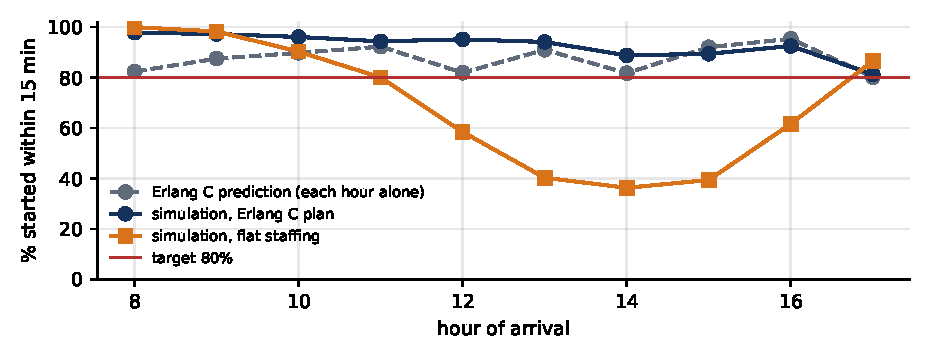
\includegraphics[width=0.9\linewidth]{../figs/lab6_sla.pdf}
\caption{Share of orders started within 15 minutes, by hour of arrival: Erlang C prediction versus simulation.}\end{figure}
\interp{For a 15-minute promise Erlang C asks for 44 picker-hours. Simulation says the plan delivers 92\% overall
($\pm1.5$), better than the formula predicts in most hours, because the day starts empty and Erlang C assumes each hour
has reached steady state. The exception is the last hour (81\%): backlog from the afternoon carries over. Flat
staffing with 40 hours (four pickers all day) looks almost as cheap but collapses to 62\%, with a 90th-percentile wait of 46
minutes. Matching staff to the arrival profile matters more than the total number of hours.}

\step{Step 3: The December order, optimised for uncertainty}
\codeout{lab6_s3}{Two-stage stochastic programme for four shelf-stable products sharing 7\,000 litres of storage.}
\interp{The deterministic plan orders the full forecast of oil, milk and sardines and fills the store room with rice
(7\,000 litres). The stochastic plan orders less of everything and leaves 1\,000 litres empty. That looks timid, but
on 20\,000 fresh scenarios it earns 772\,000\xaf\ against 705\,000\xaf: a VSS of 67\,000\xaf, or 9.5\%. With a
forecast error of 40\% and clearance at 40\% of cost, every unit beyond the median is more likely to be cleared at a
loss than sold. The EVPI of 346\,000\xaf\ is the ceiling on what better December forecasting could ever earn for these
four products in this store: worth a serious effort, and a number to quote when someone proposes a forecasting
project.}

\paragraph{So what (model answer)} \emph{To start 80\% of orders within 15 minutes, staff two pickers at 8:00 rising to
six over lunch: 44 picker-hours a day delivers about 92\%. Flat staffing at four pickers saves four hours but cuts
service to 62\%. For December, order below forecast for every shelf-stable product; modelling forecast uncertainty is
worth about 67\,000\xaf\ per store this month.}

% ------------------------------------------------------------------ EXERCISES
\section{Exercises}
\begin{enumerate}[label=\textbf{6.\arabic*},leftmargin=2.4em]
\item \emph{(M/M/1)} A single cashier serves 50 customers an hour on average (mean 1.2 minutes each); customers arrive
at 45 an hour. Compute $\rho$, $L_q$ and $W_q$. What happens to $W_q$ if arrivals rise 10\%?
\item \emph{(Erlang C, Mboa clinic)} From \texttt{clinic.csv}, estimate arrivals between 9:00 and 10:00 and the mean
service time. How many doctors keep the probability of waiting below 30\%? Below 10\%?
\item \emph{(Pooling)} Two separate M/M/1 queues each with $\rho=0.8$, or one M/M/2 queue with the same total load:
compare $W_q$. Explain to a bank branch manager.
\item \emph{(Cost of delay)} In Step 1, suppose each minute an order waits beyond 30 minutes costs \pounds0.20 in lost
goodwill and a picker-hour costs \pounds12. Find the cost-minimising pickers at noon.
\item \emph{(Simulation)} In Step 2, give pickers a 30-minute lunch break in rotation between 12:00 and 14:00. How much
does service fall, and which hour suffers? Use common random numbers.
\item \emph{(Simulation)} Replace the empirical service times with exponential ones of the same mean. Does the result
change? Relate to Allen--Cunneen.
\item \emph{(SAA)} In Step 3, solve with $K=50,100,300,1000$ scenarios and plot the out-of-sample profit. How many
scenarios are enough?
\item \emph{(VSS)} Recompute VSS with forecast CV 0.2 and clearance at 70\% of cost. When is a deterministic plan good
enough?
\end{enumerate}

\section{Take-home assignment 6 and CA3 preparation}
Build a SimPy model of the Mboa clinic (\texttt{clinic.csv}) with the real hourly arrival pattern and service times.
Find the cheapest doctor roster (in 4-hour blocks) that sees 90\% of patients within 30 minutes. Report the roster,
its cost at 6\,000\xaf\ per doctor-hour, and a 95\% confidence interval for the service level. CA3 will ask you to
formulate an allocation model and test it under uncertainty in two hours.
